\setboolean{IsHalfPage}{false}%
\setboolean{IsHalfPageLeftCol}{false}%
\setboolean{IsHalfPageRightCol}{false}%
\def\ChapterTitle{%
	X Transit Hub
}
\def\ChapterUrl{%
	https://arnottferels.github.io/work/x-transit-hub
}
\def\ChapterDescription{%
	Walkability Model Using Dynamic Multilayer Method in Transit Hub Design
}
\def\ChapterDetailsLine{%
	Master's Thesis -- 2023 | Urban Research; Transit Design; Public Space; Computation | West Jakarta, Indonesia
}
\def\ChapterDetailsTabular{%
	\begin{tabular}{@{}ll}
		\textbf{Type}     & Individual work                                                                                 \\
		\textbf{Software} & Rhino, Grasshopper, Wallacei, Quelea, Caribou, Arachne, Kangaroo 2, Twinmotion, Adobe Photoshop \\
		\textbf{Advisor}  & Aswin Indraprastha                                                                              \\
		\textbf{Jury}     & M. Donny Koerniawan, Heru W. Poerbo                                                             \\
		\textbf{URL}      & \textcolor{blue}{\footnotesize\texttt{\href{\ChapterUrl}{\ChapterUrl}}}                         \\
	\end{tabular}
}
\def\ChapterAbstract{%
	This thesis delves into the challenges, methodologies, and solutions associated with the design of a transit hub (TH) in Jakarta that integrates both public transportation and public spaces (PS). A Dynamic Multi-Layer (DML) method addresses these intricate challenges by examining traffic density, simulating pedestrian movements, and optimizing for multiple objectives, such as minimizing distance to PS and reducing the total number of PS. The ultimate solution serves as a blueprint for the TH design, emphasizing human mobility, connectivity, and greenery.
}
\def\ChapterFrontmatter{%
	\chapter*{\ChapterTitle}\addcontentsline{toc}{chapter}{\ChapterTitle}
	\ChapterSetTocAddData{\ChapterDetailsLine}
	\ChapterSetDetailsData{\ChapterDescription}{\ChapterDetailsLine}{\ChapterDetailsTabular}
	\RuleAbstract%
	\ChapterAbstract
}
\StartTwoColumnLayout
\ChapterFrontmatter
\section*{%
  Design
 }
\begin{figure}[H]
	\centering
	\includesvg[width=\linewidth]{src/graphics/x-transit-hub--section-aa.svg}
	\caption*{%
		Cross-section: West-to-east axis (Section A-A)
	}
	\label{
		fig:x-transit-hub--section-aa
	}
\end{figure}

\vfill
\begin{figure}[H]
	\centering
	\includesvg[width=\linewidth]{src/graphics/x-transit-hub--section-bb.svg}
	\caption*{%
		Cross-section: West-to-east axis (Section B-B)
	}
	\label{
		fig:x-transit-hub--section-bb
	}
\end{figure}

\vfill
\begin{figure}[H]
	\centering
	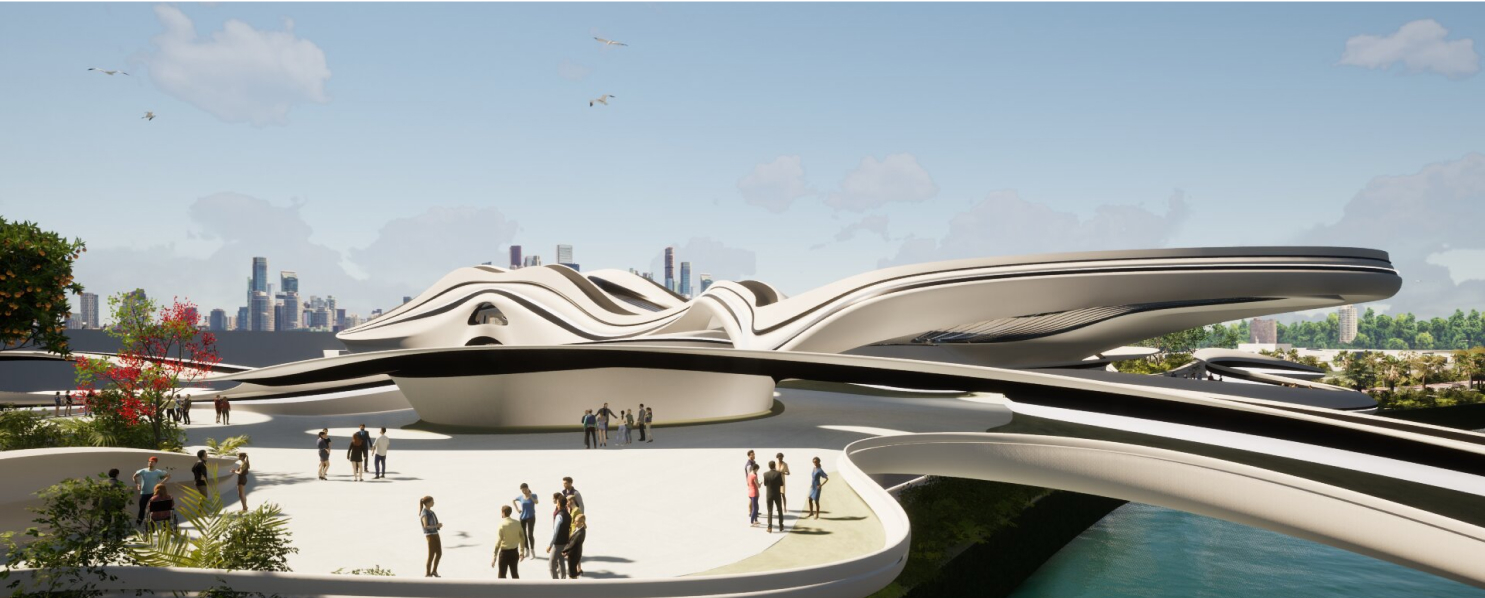
\includegraphics[width=\linewidth]{src/graphics/x-transit-hub--perspective.jpg}
	\caption*{%
		\parbox{0.7\linewidth}{%
			\centering
			A perspective showing activities in green spaces and the extraction of major axis shapes from patterns using the Dynamic Multi-Layer (DML) method (explained on the following pages).
		}
	}
	\label{
		fig:x-transit-hub--perspective
	}
\end{figure}

\columnbreak%
\begin{figure}[H]
	\centering
	\includesvg[width=\textwidth, height=\textheight, keepaspectratio]{src/graphics/x-transit-hub--exploded-axonometric.svg}
	\label{
		fig:x-transit-hub--exploded-axonometric
	}
\end{figure}
%
\newpage
\section*{%
  Methodology
 }
\begin{figure}[H]
	\centering
	\includesvg[width=\linewidth]{src/graphics/x-transit-hub--methodology.svg}
	\label{
		fig:x-transit-hub--methodology
	}
\end{figure}

DML method framework. These are: traffic analysis (1), dynamic crowd modeling (2), the smoothing and simplification of multiple paths (3), multi-objective optimization (4~and~5), and solution clustering and selection (6).
\vfill
\subsubsection*{Data Gathering \& Modeling Preparation (Traffic Analysis)}
\begin{center}
	\begin{minipage}{0.85\linewidth}
		\begin{figure}[H]
	\centering
	\includesvg[width=\linewidth]{src/graphics/x-transit-hub--routes-taxonomy.svg}
	\caption*{%
		The taxonomy of routes in Kalideres is based on traffic observations and pivotal variables, creating route segmentation.
	}
	\vspace*{\baselineskip}%
	\label{
		fig:x-transit-hub--routes-taxonomy
	}
\end{figure}

		\begin{figure}[H]
	\centering
	\includesvg[width=\linewidth]{src/graphics/x-transit-hub--routes-scoring.svg}
	\caption*{%
		Route scoring is based on route segmentation.
	}
	\vspace*{\baselineskip}%
	\label{
		fig:x-transit-hub--routes-scoring
	}
\end{figure}

		\begin{figure}[H]
	\centering
	\includesvg[width=\linewidth]{src/graphics/x-transit-hub--point-map-agent-based.svg}
	\caption*{%
		Point-map with agents (AR, AT) and targets (T1, T2).
	}
	\label{
		fig:x-transit-hub--point-map-agent-based
	}
\end{figure}

	\end{minipage}
\end{center}
In Layer 1, Google Maps Typical Traffic (GMTT) data (6~AM — 10~PM) analyzed congested routes and pedestrian movements. On-ground mapping and digital tools like Rhino, Grasshopper, and Caribou played crucial roles. GMTT data, ranked 1~to~3 for traffic densities, guides Layer 2 in identifying attraction points and key agents.
\columnbreak%
\subsubsection*{Predicting Dynamic Model of Complex System}
\begin{figure}[H]
	\makebox[\linewidth][c]{%
		\includesvg[width=1.15\linewidth]{src/graphics/x-transit-hub--abm-superimpose.svg}
	}
	\caption*{%
		Aggregated results from agent-based simulations in Iterations 1, 2, and 3, illustrating crowd movement in the virtual environment.
	}
	\label{
		fig:x-transit-hub--abm-superimpose
	}
\end{figure}
%
\vfill
\begin{table}[H]
	\renewcommand{\arraystretch}{1.5}
	\centering
	\small
	\begin{tabularx}{\linewidth}{@{}X@{\hspace{0.5cm}}X@{\hspace{0.5cm}}X@{}}
		\textbf{Solo Commuting (Iteration 1)}                                                                                                     & \textbf{Solo Walking (Iteration 2)} & \textbf{Group Touring (Iteration 3)} \\
		Designed for students and working professionals, this configuration activates \texttt{Wandering} while deactivating \texttt{Align Force}. &
		Tailored for leisure walkers, this configuration deactivates both \texttt{Wandering} and \texttt{Align Force}.                            &
		Configured for group tours, this setup deactivates \texttt{Wandering} and activates \texttt{Align Force}.                                                                                                              \\
	\end{tabularx}
\end{table}
\vfill
In Layer 2, utilizing agent-based simulation, agent configurations for AR, AT, T1, and T2 were derived from insights in Layer 1 through three iterative refinements. Configurations include Solo Commuting (students, professionals), Solo Walking (leisure walkers), and Group Touring (group tours). After 300 steps using tools like Grasshopper and Quelea, agent trajectories were evaluated, revealing patterns. Iteration 1 facilitates smooth navigation, Iteration 2 shows agent clustering in bustling zones, and Iteration 3 sees dense congregation around T1 and T2, indicating congestion hotspots. The simulations provide insights for urban renewal projects and infrastructure enhancements.
\columnbreak%
\subsubsection*{Simplifying the Trails}
\vspace*{-0.5\baselineskip}%
\begin{figure}[H]
	\centering
	\includesvg[width=\linewidth]{src/graphics/x-transit-hub--ls.svg}
	\label{
		fig:x-transit-hub--ls
	}
\end{figure}

In Layer 3, data from three Layer 2 iterations is smoothed using Laplacian technique, maintaining even spacing. Modal points undergo iterative modifications, aligning with the 10th iteration and defining mesh space with shortest path algorithm (SPA). Aligned with TOD Standard 3.0 and SDGs 11 for robust transportation infrastructure and urban design.
\vfill
\subsubsection*{Defining the Objectives}
\vspace*{-\baselineskip}%
\begin{figure}[H]
	\centering
	\includesvg[width=\linewidth]{src/graphics/x-transit-hub--spa.svg}
	\label{
		fig:x-transit-hub--spa
	}
\end{figure}

In Layer 4, SPA and A-star algorithms converge, paving the way for optimization in Layer 5. The computational agility of A-star transforms input lines into a refined foundational mesh using TriRemesh in Kangaroo2. This mesh serves as trails for SPA, with T1 and T2 as terminal markers (nodes).
\vfill
\subsubsection*{Optimizing the Objectives}
\vspace*{-\baselineskip}%
\setlength{\columnsep}{0.25cm}%
\begin{multicols}{2}
	\begin{figure}[H]
	\centering
	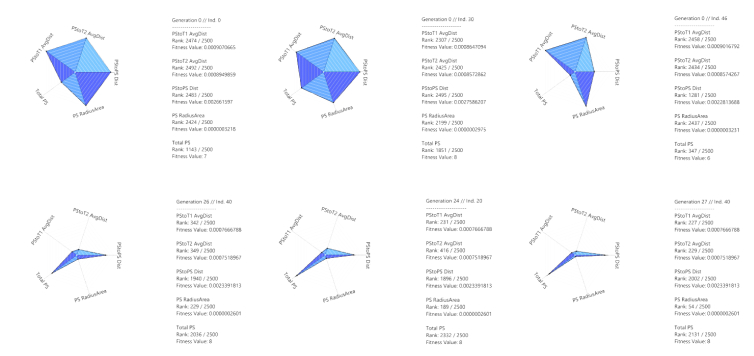
\includegraphics[
		height=3.5cm,
		keepaspectratio
	]{src/graphics/x-transit-hub--moo-dfc.jpg}
	\caption*{%
		Diamond Fitness Chart (DFC) traces optimization progress.
	}
	\vspace*{-0.5\baselineskip}%
	\label{
		fig:x-transit-hub--moo-dfc
	}
\end{figure}

	\begin{figure}[H]
	\centering
	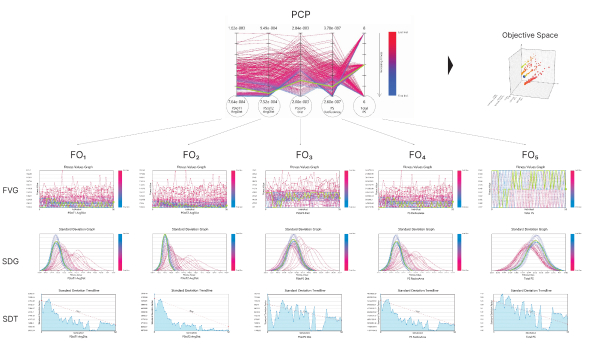
\includegraphics[
		height=3.5cm,
		keepaspectratio
	]{src/graphics/x-transit-hub--moo-graph.jpg}
	\caption*{%
		PCP, FVG, SDG, and SDT offer a comprehensive view of generation.
	}
	\vspace*{-0.5\baselineskip}%
	\label{
		fig:x-transit-hub--moo-graph
	}
\end{figure}

\end{multicols}
\vfill
\begin{figure}[H]
	\centering
	\includesvg[width=\linewidth]{src/graphics/x-transit-hub--moo-process.svg}
	\label{
		fig:x-transit-hub--moo-process
	}
\end{figure}

In Layer 5, EMOO simulation, driven by NSGA-II, aims for advanced outcomes. Fitness Objectives (FO) prioritize average route distances, Voronoi radii area, and total potential Public Space (PS) count, emphasizing uninterrupted mobility, placemaking, and urgency. The study, evaluating 2,500 potential solutions with Wallacei, confirms the method's effectiveness, setting the stage for the next layer to select the best design guideline through solution clustering techniques.
\columnbreak%
\subsubsection*{Clustering \& Selecting the Best Solution}
\begin{figure}[H]
	\centering
	\includesvg[width=\linewidth]{src/graphics/x-transit-hub--clustering-method.svg}
	\vspace*{0.5\baselineskip}
	\caption*{%
		A method for clustering the set of solutions into the best solution. It is called the Selection Clustering (SC) method.
	}
	\vspace*{0.5\baselineskip}
	\label{
		fig:x-transit-hub--clustering-method
	}
\end{figure}

In Layer 6, the focus is on detailed clustering of the extensive set of 2,500~solutions using the SC method. The objective is to determine the most pertinent design guidelines. This method unfolds over five phases, collectively termed ``solution clustering,'' fine-tuned to choose the most suitable solution for the study.
\vfill
\begin{figure}[H]
	\centering
	\includesvg[width=\linewidth]{src/graphics/x-transit-hub--best-solution.svg}
	\caption*{%
		Best solution -- Gen47~Idv30.
	}
	\vspace*{0.5\baselineskip}
	\label{
		fig:x-transit-hub--best-solution
	}
\end{figure}

Upon reevaluating the chosen solution (Gen47~Idv30), the initial criteria set for all FOs were revisited. Ideally, these criteria should align with the highest standards, particularly when compared to the clusters identified in Layer 6. Achieving the set goals for each FO is crucial. The assessment reveals that all objectives have been met, positioning the selected solution as a leading design guideline for the TH in the first section of this portfolio. Additionally, this solution serves as a blueprint for future planning of PS in the context.
\section*{%
  Finding
 }
In the Dynamic Multi-Layer (DML) methodology, Walkability Model (WM) is employed to track agent movement effectively, distinguishing between primary and secondary movement patterns. This approach, combined with Agent-Based Modeling (ABM), provides valuable insights for designing TH and PS. The use of WM plays a crucial role in understanding the walkable aspects of urban spaces, aiding in the formulation of design guidelines.
\EndTwoColumnLayout
\newpage
